\ifdefined\included
\else
\setcounter{chapter}{7} %% Numéro du chapitre précédent ;)
\dominitoc
\faketableofcontents
\fi

\chapter{Beyond binary relations in the REG}
\minitoc
\label{chap:7}

A number of works trend to semantically represent and describe robots' actions and tasks using ontologies. However, each representation has its own specificities, depending on the system it is used on and the exploitation it aims to enable. While our description of past activities fits our needs and our task planner, having a REG algorithm constrained by this latter is problematic. In this chapter we explore the use of n-ary relation, a common, even not yet standard, way to represent complex knowledge as actions. With the analysis of such a pattern, we present a novel REG approach, supporting the use of past activities, but also any complex knowledge represented through n-ary relations.

The contribution presented in this chapter is a preliminary work aiming to consider the limitations encountered by the contribution of the previous chapter. The proposed algorithm remains fully compatible with the previous one and hence we directly compare their performance. While it has not been the subject of direct experimentation on the robot, it should be usable as a drop-in replacement of the previous one. This section deviates a little from the field of \acrshort{hri} to be more anchored in artificial intelligence. However, the ability to generate entity referencing in a more generic way is paramount for a robot to interact with humans. 

\section{Introduction}

Representing the whole complexity of the knowledge composing our world into a machine-readable language is a central issue in artificial intelligence. Coming from the Semantic Web, we saw that the use of an ontology through RDF-based languages succeeded in establishing itself in the field of artificial intelligence and therefore robotics. However, what is often viewed as a limitation of ontologies is its capability to only represent unary and binary relations. Binary relations such as \textit{``Sean Connery has the British nationality''} are described through the form of triplets \textit{(sean\_connery, hasNationality, british)}. Unary relations such as \textit{``Sean Connery is an actor''} can then be transformed into binary relations through the addition of dedicated predicates \textit{(sean\_connery, isA, Actor)}. However, the description of more complex relations involving more than two entities is much more challenging using this kind of representation.

Taking the example of Sean Connery\footnote{In the case you do not know who is Sean Connery feel free to take another actor that you like but you will have to adapt the entire example.}, if we want to refer to him\footnote{Obviously we want to refer to him without his name since we consider a person having recognized himself in the previous note.}, we could state that he is the actor playing the role of James Bond \textit{(sean\_connery, hasPlayedRole, james\_bond)}. However, other actors played this role. We could also say that he is the actor playing in the film Goldfinger \textit{(sean\_connery, hasPlayedIn, goldfinger)} but once again others do. We could finally explain that he is the actor playing the role of James Bond and playing in the film Gold Finger. However, limiting us to the use of binary relations modify the exact information. A more accurate description would be that he is the actor playing the role of James Bond in the film Gold Finger. Here we see the necessity of relations involving more than two entities. In our example, we need to link the three entities that are the actor ``Sean Connery'', the role ``James Bond'', and the film ``Gold Finger''. Together, they describe a performance. Without being explicitly linked, these three pieces of information would not represent the performance. Moreover, without these links, we could give an explanation such as the actor playing the role of James Bond and playing in the film Rising Sun. Both pieces of information are true but do not make sense together.

To refer to an entity, being an object or an agent, such complex relations could be useful but have to be managed carefully to keep the link between each binary relation composing it. In the light of this consideration, we can observe that the description of past agent tasks used in the previous chapter is based on the same principle. Where we refer to Sean Connery through his role and the film he plays in, we have described the knife through the vegetable it was used to cut and the agent who used it. However, depending on the context of the conversation, it is not always necessary to use all the binary relations of such a complex relation. We may need only one. Trying to list the actors having the honorific title of ``Sir'', the referring expression \textit{``The man having played James Bond''} could be sufficient. In the same way, to designate the knife, the sentence \textit{``The knife you cut with''} could also be sufficient in some context.

In this chapter, we will try to generalise the \acrshort{reg} algorithm to deal with non-binary relations and pass over the limitations of the previous chapter. The algorithm has to be more generic and should no more have any apriori of concepts and properties of the used ontology.
First, we review the literature concerning the representation of non-binary relations in ontology. Then, we define what we will call a \acrlong{cr} and how we can represent it. The modified algorithm is then detailed before ending with an efficiency comparison regarding the original version and the extended one.

\section[Related work]{Related work: A richer knowledge representation with n-ary relations}

A fundamental feature of relations is their \textbf{arity}. It is the number of individuals they involve~\cite{giunti_2019_representing}. In this sense, unary relations involve only one entity while binary relation involves two entities\footnote{The entities involved in a relation do not have to be distinct. If the same entity is used twice in the same relation the relation is still a binary relation}. What interests us here is n-ary relations with arity $n > 2$.

Well before being treated for ontology usage, that it is in RDF or OWL, several approaches have been proposed in the field of Artificial Intelligence through the use of semantic network\footnote{Here we close the loop with the hypothesis by Collins and Quillian of the structure of the semantic memory to be like a semantic network.}~\cite{brachman_1979_epistemological, sowa_2014_principles}. Deliyanni and Kowalski~\cite{deliyanni_1979_logic} were the first to explicitly treat the representation of n-ary relations with arity $n > 2$. They propose a semantic network composed of an element representing the relation itself. In this way, they have represented the assertion ``\textit{John gives the book to Mary}'' with five nodes and four arrows as illustrated in Figure~\ref{fig:chap7_sem_net}. The central node \textit{el} allows linking the four elements of the assertion using only binary relations. The approach is today know as \textbf{relation reification} and has been used in many applications~\cite{gangemi_2008_norms, welty_2006_reusable}.

\begin{figure}[ht!]
\centering
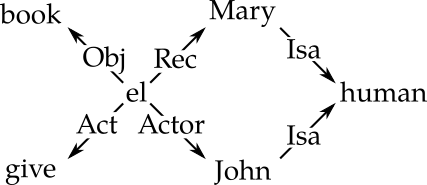
\includegraphics[scale=0.5]{figures/chapter7/semantic_net.png}
\caption{\label{fig:chap7_sem_net} The semantic network used to represent the assertion ``\textit{John gives the book to Mary}''. The element \textit{el} is used to represent the global event.}
\end{figure}

The general idea used in all the proposed approaches since Deliyanni is thus the creation of a \textbf{relation-class}. From this class, we create an instance of it that represents a specific n-ary relation. Then $n$ binary relations are created to link the $n$ entities to the relation-class instance. For example, in Figure~\ref{fig:chap7_sem_net}, the instance of the relation-class is $el$ and the n-ary relation is the set of the four relations $el$ is involved in. For a more global view of the different proposed patterns, you can refer to the survey~\cite{gangemi_2013_multi}.

For the use in an ontology, no standard pattern has been approved so far by the W3C. However, a Working Group Note has been proposed for the standardisation of such relations in RDF and OWL~\cite{w3c_2006_defining}. In the note, two patterns are introduced with two variants for the first one.

\paragraph{Pattern 1 (without subject):} The first pattern is based on the introduction of a new class for relation and is illustrated by the relation reification in Figure~\ref{fig:chap7_w3c_p2}. The class \textit{Purchase} is a relation-class and its instance \textit{purchase\_1} is linked to the entities of the relation. This pattern is said to be \textbf{without subject} as all the relations are oriented from the relation-class instance to the other entities.

\begin{figure}[ht!]
\centering
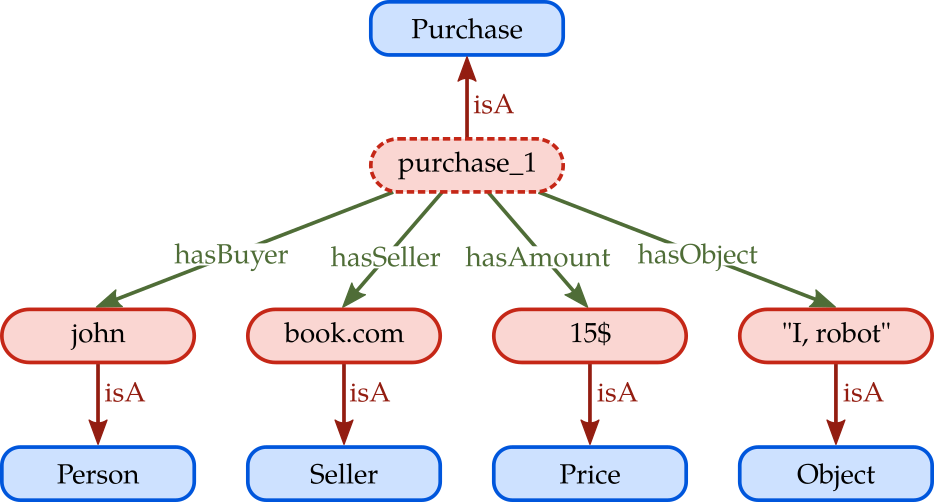
\includegraphics[scale=0.45]{figures/chapter7/w3c_p2.png}
\caption{\label{fig:chap7_w3c_p2} Ontological pattern 1 without subject proposed by the W3C Working Group. The described assertion is ``John buys ''I, robot`` from books.com for \$15''.}
\end{figure}

\paragraph{Pattern 1 (with subject):} A variation of the first pattern is illustrated in Figure~\ref{fig:chap7_w3c_p1}. This variation is said to be \textbf{with subject}. The assertion described here is ``Christine has a tumor with high probability''. Here the subject of the relation is Christine. It is represented in the pattern by a relation oriented from Christine to the instance of the relation-class while the others are in the usual orientation. Such variation can be reproduced with the previous one by defining inverse relations. Defining the relation \textit{isBuyer} and \textit{isObject}, either John or the book can be the subject of the relation represented by \textit{purchase\_1}.

\begin{figure}[ht!]
\centering
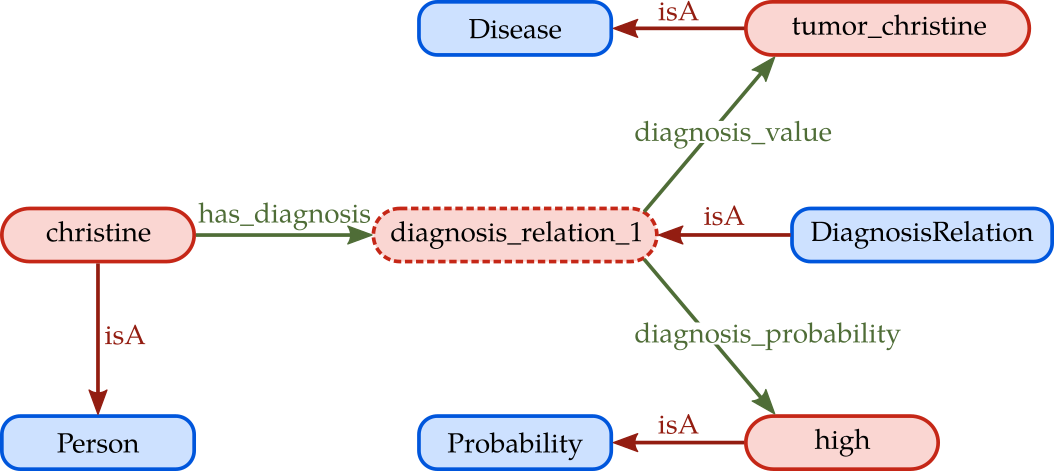
\includegraphics[scale=0.4]{figures/chapter7/w3c_p1.png}
\caption{\label{fig:chap7_w3c_p1} Ontological pattern 1 with subject proposed by the W3C Working Group. The describe assertion is ``Christine has tumor with high probability''.}
\end{figure}

\paragraph{Pattern 2:} The second pattern aims at representing lists, which was not possible with the first pattern. With the previous pattern, it is assumed that the properties involved in the binary relation are only used once to identify uniquely each element of the relation. Wanting to represent the assertion ``United Airlines flight 3177 visits the following airports: LAX, DFW, and JFK'' the first pattern would not be adapted. With this other pattern, we create several instances of the relation-class each linked to the next and to an entity of the n-ary relation as illustrated in Figure~\ref{fig:chap7_w3c_p3}. Because one of the binary relations go from an entity of the relation to an instance of the relation-class, it is said to be with a subject. This second pattern is dedicated to the description of lists.

\begin{figure}[ht!]
\centering
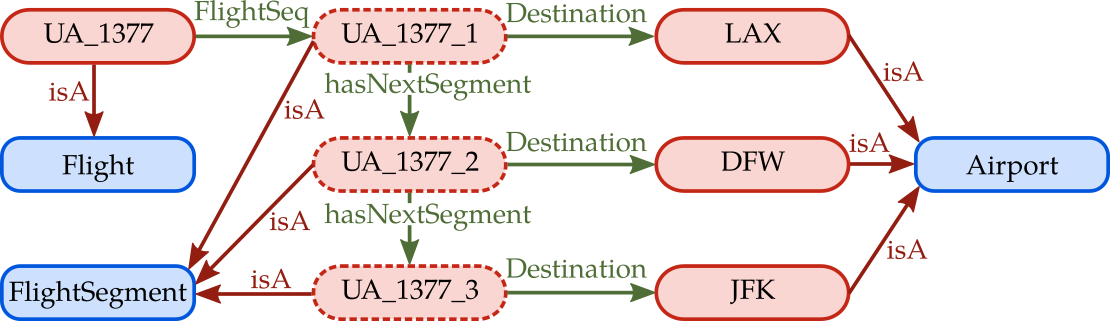
\includegraphics[scale=0.4]{figures/chapter7/w3c_p3.png}
\caption{\label{fig:chap7_w3c_p3} Ontological pattern 2 with subject proposed by the W3C Working Group. The describe assertion is ``United Airlines flight 1377 visits the following airports: LAX, DFW, and JFK''.}
\end{figure}

\section{Through the use of compound relations}

In the rest of the chapter, we consider the n-ary relations with arity $n > 2$ under the name \textbf{\acrfull{cr}} because of the composition of binary relations to represent them on the principle of reification. The term relation will be used to speak about binary relations. We first define what is a \acrshort{cr} with respect to ontology definition and based on the first pattern without subject, proposed by the Working Group Note. Then, we present an algorithm to pre-process \acrfull{cr}s with the objective to facilitate their use in the \acrshort{reg} algorithm.

\subsection{Defining a compound relation}

To define the structure of a \acrlong{cr} we take the example of the purchase made by John on the website book.com to buy the book ``I, Robot'' at 15\$, illustrated in Figure~\ref{fig:chap7_w3c_p2}. This statement is graphically represented in Figure~\ref{fig:chap7_cr}a and the underlying pattern in Figure~\ref{fig:chap7_cr}b. To represent the compound relation, we start by creating a virtual entity (the instance of the relation-class) that will be the common link for all the relations involved in the compound relation. We call this entity the \textbf{\acrfull{ce}}. It is the dotted entity on Figure~\ref{fig:chap7_cr}, respectively $purchase\_1$ and $\indiv_c$. We consider as being part of the \acrshort{cr} all the relations for which the \acrshort{ce} is the subject: $(purchase\_1, has\_buyer, john)$. 

\begin{definition} [Compound Relation]
\label{the:compound_relation}
For any $\indiv_c$ being a Coumpound Entity, a Coumpound Relation is defined by $R_c = \{ \relation_i\ |\  \relation_i = (\indiv_c, \property_i, \indiv_i) \in \relationset\}$ meaning the set of relations composing it.
\end{definition}

\begin{figure}[ht!]
\centering
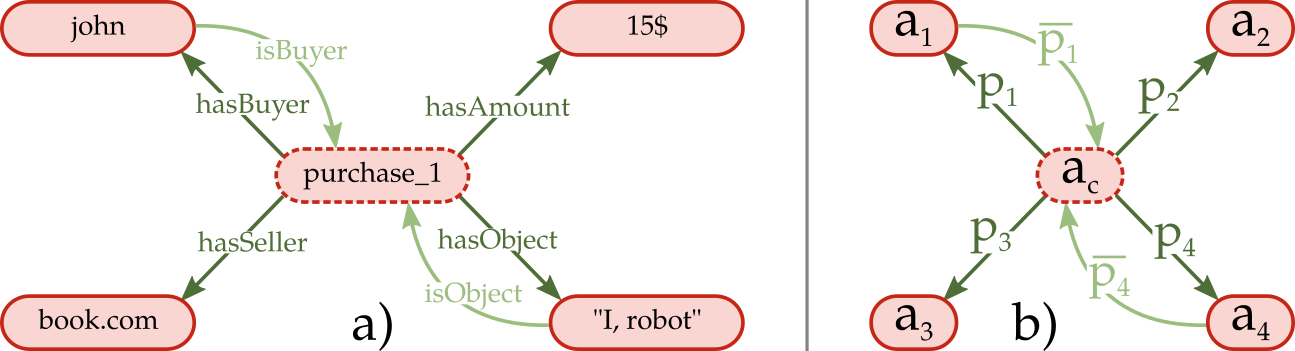
\includegraphics[width=\textwidth]{figures/chapter7/CR.png}
\caption{\label{fig:chap7_cr} The graphical representation of compound relations. The dotted entity at the center of each representation is the so-called compound entity. The outgoing edges are the properties involved in the compound relation. The entering and faded edges are the corresponding inverse properties if any. The compound relation a) describes the purchase made by \underline{John} on the website \underline{book.com} of the book \underline{``I, Robot''} at \underline{15\$}. The compound relation b) is the underlying pattern of the previous example.}
\end{figure}

Regarding the previous definition, because any entity of an ontology could be considered as a \acrshort{ce}, many sets of relations without a real link could be considered as a \acrshort{cr}. To solve it, we could define an upper class common to all the \acrshort{ce}, meaning the upper \textit{RelationClass}. However, in the context of the \acrshort{reg}, what better defines a \acrshort{cr} is that to speak about one of its involved entities using the \acrshort{cr}, we have to use other relation of the \acrshort{cr}. In other words, to speak about Sean Connery using the role of James Bond, we have to speak about ``Gold Finger'' rather than ``Murder on the Orient Express'' because even if he played in both films, he played the said role only in the first-mentioned film. Conversely, the relation representing his nationality can be used independently to other relations. To represent this verbal link, Giunti et .al \cite{giunti_2019_representing} introduce a \textit{parametric pattern} on top of n-ary relations (Compound Relations). Their parametric pattern for the purchase example is the following : \textit{``() bought () from () for ()''}. While as humans we easily identify the place of each entity in the pattern, it is a more complex task for machines. This choice of pattern is explained by their complex representation where they assign a position to each involved relation. Regardless of the representation complexity, this kind of pattern raises two issues. First, the pattern describes the entire \acrshort{cr} and does not aim to describe one of the involved entity through the \acrshort{cr} (e.g. ``\textit{() who bought () from () for ()}''). Second, the pattern necessarily involves all the relations composing the \acrshort{cr}, while in the context of the \acrshort{reg}, we could only need a part of them (e.g. \textit{``() who bought ()}'' if John is the only one who bought this book in the present context).

\subsection{A lightweight representation of the verbal link}

To represent the verbal link, we also choose to use parametric patterns, patterns for short, defined as labels in the ontology. However, to know the position of each binary relation among the place-holders, we choose to integrate into the patterns the properties which can be used to form the relations composing the \acrshort{cr}. Considering the example of Figure~\ref{fig:chap7_cr}, our patterns have the following form : $\{?hasObject\}\ bought\ on\ \{hasSeller\}\ by\ \{hasBuyer\}$. In the following, we will prefer the more generic patterns $\{?\property_4\}\ bought\ on\ \{\property_3\}\ by\ \{\property_1\}$.

Given a compound entity $a_c$ with the previous label, to generate a referring expression using it, the place-holder $\{\property_3\}$ should be replaced by a referring expression of an entity $\indiv_i$ where $\indiv_i$ is the object of a triple $(\indiv_c,\ \property3,\ \indiv_i)$. Because we assume that a property can only appear once in a \acrshort{cr}, we know that there is only one such object $\indiv_i$. In our example, we have $\indiv_i = \indiv_3$ for the $a_c$ \acrshort{ce}.
In this way, without predefined order, an algorithm can easily replace the place-holders by the \acrshort{re} of the entities $\indiv_i$ of the relations $(\indiv_c, \property_i, \indiv_i)$ of the \acrshort{cr}. With the example pattern, the resulting sentence would be: \textit{``The book bought on book.com by John''}.

Since we are in the context of \acrshort{reg}, the \acrshort{cr} will be used as a reference to one of the entities involved in it. This specific entity is called the \textbf{subject entity} of the \acrshort{cr}. In our example pattern, the subject entity is $a_4$, meaning the bought book. A \acrshort{cr} can thus have multiple labels (i.e. patterns) depending on the subject of the pattern and the involved relations in the verbal link. With our example, we might also want to refer to the website or the buyer. Moreover, if John purchased multiple books on the given website, we might need to refer to the book's price to refer to the book.

For a subject entity to exist, an inverse property $\overline{\rm \property_i}$ must exist in the way that $(\property_i, \overline{\property_i}) \in \invset$ and $\relation_i = (\indiv_i, \overline{\property_i}, \indiv_c) \in \relationset$. If $\indiv_i$ is the subject entity, $\property_i$ is thus the \textbf{subject property} of the \acrshort{cr} and is prefixed with a question mark in the pattern. In the example of Figure~\ref{fig:chap7_cr}, only $\indiv_1$ and $\indiv_4$ (resp. John and the book) can be subject of the \acrshort{cr}. In other words, only these entities can be referred through the use of this \acrshort{cr}. Among all the labels available to speak about the \acrshort{cr}, the usable ones to speak about an entity are the ones for which the corresponding property is the subject property (i.e. prefixed by a question mark in the patterns). This choice to not consider the first in the pattern has been made to be adapted to any language. Among the possible labels of Listing~\ref{lst:chap7_john_labels}, the patterns L1 to L5 could thus be used as a reference for $\indiv_4$ (the book in our example) while the patterns L6 and L7 could be used as a reference for $\indiv_1$ (John in our example).

\begin{lstlisting}[frame=single, caption={ A part of the label set of the purchase compound relation.}, label={lst:chap7_john_labels}, captionpos=b, style=Labels, mathescape=true]
L1 - {?$p_4$} bought on {$p_3$} at {$p_2$}
L2 - {?$p_4$} bought by {$p_1$}
L3 - {?$p_4$} bought on {$p_3$} by {$p_1$}
L4 - {$?p_4$} bought at {$p_2$} on {$p_3$} by {$p_1$}
L5 - {$?p_4$} bought at {$p_2$} by {$p_1$}
L6 - {$?p_1$} who bought {$p_4$}
L7 - {$?p_1$} who bought {$p_4$} on {$p_3$}
\end{lstlisting}

The labels are not directly applied to the \acrshort{ce} but to the class it inherits. This means that all the entities inheriting from a class having at least one label of the form of the previously introduced pattern, are \acrshort{ce}. In a way, we define here a relation-class but only through the use of labels.

\begin{definition} [Compound Entity]
\label{the:compound_entity}
Given a pattern $\omega$, an entity $\indiv_c$ is a \acrlong{ce} iff $\exists \class \in \classset | (\indiv_c, \class) \in \inheritset \land \omega \in \tlabel{(\class)}$
\end{definition}

An advantage of this solution is that we do not define any new specific concepts or properties in the ontology meaning that any pre-existing ontology can be updated to be used in the \acrshort{reg} process with \acrshort{cr} only by adding labels, as n-ary relations are already used.

\subsection{A strategy to explore compound relations}

To use \acrlong{cr}s in the generation of \acrlong{re}s, the \acrshort{reg} algorithm will have to explore each binary relation composing it. Moreover, to create a valid \acrshort{re}, the algorithm will have to find a combination of binary relations usable in one of the patterns of the \acrshort{cr}. However, such a number of possibilities to test with the original algorithm can engender combinatorial explosion. In a graph exploration, an important parameter to avoid a combinatorial explosion is the branching factor. For the \acrshort{reg} problem, an advantage of \acrshort{cr} is that once we introduce a \acrshort{cr} in the search algorithm we can directly know the relations involved in it. In this sub-section, our goal is thus to analyze the labels in the way to define the order in which the relations of the \acrshort{cr} will be explored by the \acrshort{reg} algorithm. By doing so, we will reduce its branching factor and thus avoid any combinatorial explosion of the \acrshort{reg} algorithm.

\subsubsection{A naive strategy to explore compound relations}

The general strategy we want to adopt is to create a sub exploration tree, representing the exploration of a \acrshort{cr}, that we will graft to the original \acrshort{reg} exploration tree. The resulting constraints we will see in the following, are that we have to insert only one relation a the time (like the \acrshort{reg} algorithm) and that the terminal nodes of the sub-trees have to be verbalisable.

Suppose we want to refer to the entity $\indiv_4$ using the compound relation embodied by the compound entity $\indiv_c$ of Figure~\ref{fig:chap7_cr}. This is made possible by the triplet $(\indiv_c,\property_4,\indiv_4)$ in the knowledge-base and its inverse $(\indiv_4, \overline{\property_4}, \indiv_c)$. Listing~\ref{lst:chap7_john_labels} presents some alternative ways in which we can verbalise entities through the \acrshort{cr}. In order to refer to $\indiv_4$, we can only use the ones where $\property_4$ is the subject property. Thus the labels L1 to L5 are the only ones that we can use. The subsets of the compound relation used by labels L1 and L3 are illustrated in Figure~\ref{fig:chap7_cr_part}.

\begin{figure}[ht!]
\centering
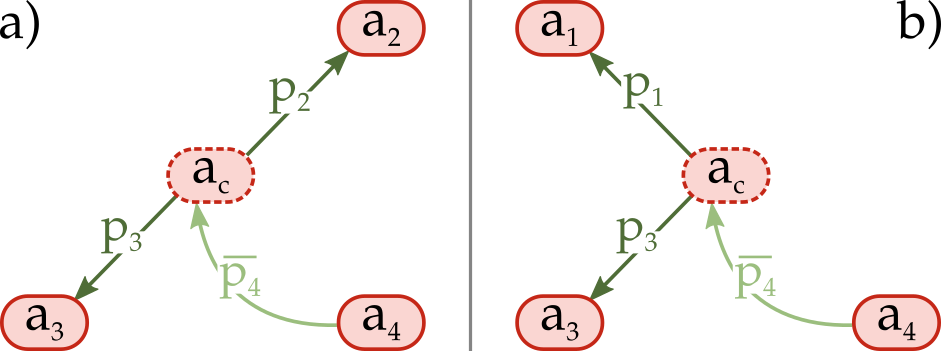
\includegraphics[scale=0.4]{figures/chapter7/CR_part.png}
\caption{\label{fig:chap7_cr_part} The parts of the compound relation used in the label patterns L1 (a) and L3 (b).}
\end{figure}

What interest us in these labels are the involved properties. Indeed, these properties will inform us about the relations to explore. From the patterns in Listing~\ref{lst:chap7_john_labels}, we know that we can use label L1 to verbalize the triple set \textit{\{($\indiv_c$,$\property_4$,$\indiv_4$) ($\indiv_c$,$\property_3$,$\indiv_3$) ($\indiv_c$,$\property_2$,$\indiv_2$)\}} and label L2 to verbalise the triple set \textit{\{($\indiv_c$,$\property_4$,$\indiv_4$) ($\indiv_c$,$\property_1$,$\indiv_1$)\}}. On the other hand, other combinations of triplets involving $a_c$ cannot be used to refer to $\indiv_4$. Therefore, we can see each label usable to refer $\indiv_4$ as a set of properties and the collection of usable labels as a family of sets. In our example, the family of sets over S is the collection:

\begin{align*}
 F\ =\ \{\{p_2\ p_3\ p_4\},
\{p_1\ p_4\},
\{p_1\ p_3\ p_4\},
\{p_1\ p_2\ p_3\ p_4\},
\{p_1\ p_2\ p_4\}\}
\end{align*}

From there, our goal is thus to create a search-tree that will conduct the exploration of the different labels of a \acrshort{cr} through the exploration of the properties composing them. This search-tree has few constraints and optimisation criteria:

\newpage

\begin{enumerate}
	\item The tree must be composed of a single root.
	\item All the descendants of a node have a common prefix of the property associated with that node. In this way, the search-tree is more precisely a trie, also called prefix tree.
	\item Walking through the tree from its root, we recompose all the subsets of the family $F$.
	\item The width of the tree must be as small as possible.
\end{enumerate}

A naive solution not minimizing the width of the tree is represented in Figure~\ref{fig:chap7_naive}a) for the purchase example. We consider the root $\property_4$ and create a branch per label. The resulting width is five. In Figure~\ref{fig:chap7_naive}b) we merge the node representing the same property at an equivalent level. It reduces the branching factor for the beginning of the exploration by the global width is the same. Switching the elements $p_2$ and $p_3$ for L4 and keeping the merging principle, we can see in Figure~\ref{fig:chap7_naive}c) that the width of the trie can be reduced to four. An advanced algorithm to build the graph could thus reduce the width of the trie.

\begin{figure}[ht!]
\centering
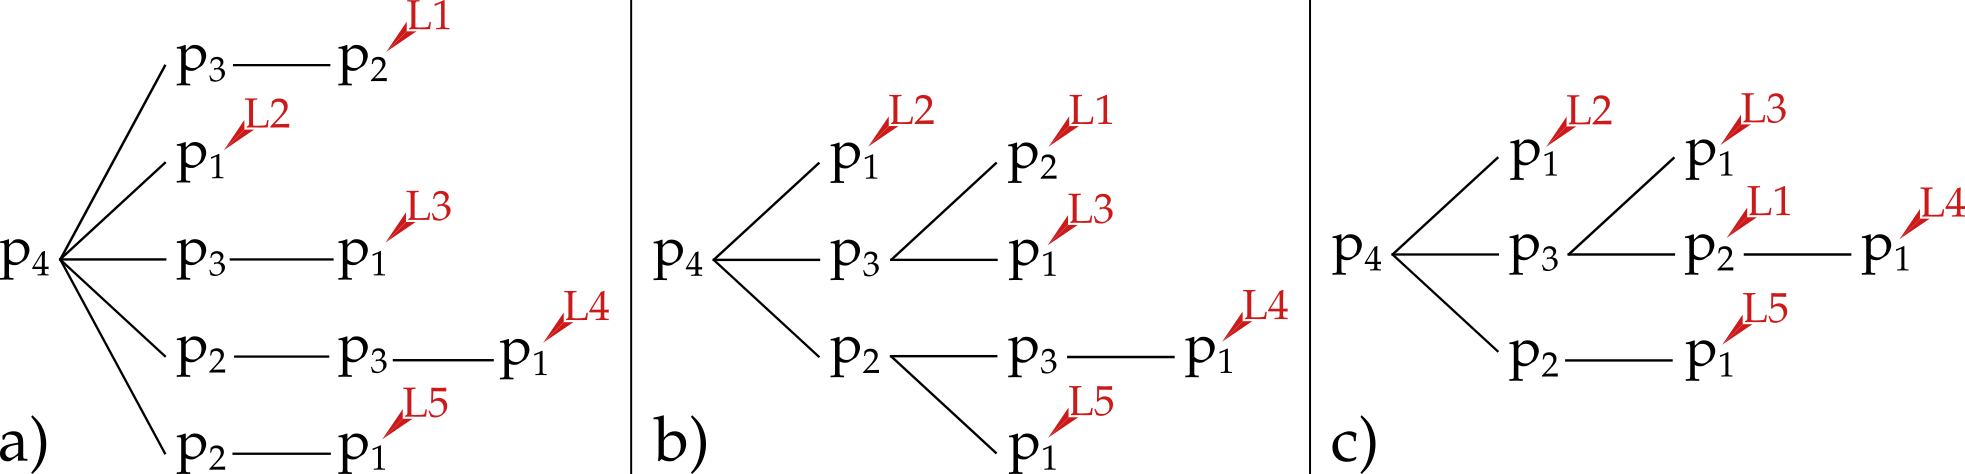
\includegraphics[width=\textwidth]{figures/chapter7/naive.png}
\caption{\label{fig:chap7_naive} Two naive trie representations of the family of subsets extracted from properties involved in the label patterns. The trie a) considers the subject property as the root of the tree and creates a branch for each label pattern respecting the order of apparition of the properties. The trie b) takes the same construction rule as the a) but merges the common children of each node. The trie c) is the same principle of b) but the elements $p_2$ and $p_3$ have been switched for L4. While the two first tries have a width of five, the last has a width of four.}
\end{figure}

\subsubsection{Advanced strategy to explore compound relations}

To find a strategy to create a trie minimizing the width, we first have to study the characteristics of the family of sets.
The first axiom that we can do on the subsets of our family is that they are neither totally ordered, as we can explore their element in any order, or partially ordered, as we can not compare their members. Therefore, we cannot use the tools of the order theory such as the Hasse diagram. Taking a look at mathematical approaches of tree-representation of set families~\cite{bui_2008_tree}, we face the problem that our set family does not respect some essential properties. For each pair $(A, B)$ of sets of $S$, we can not ensure that one of the following rules is true : $A \cap B \neq \emptyset$, $A \cap B \neq A$, or $A \cap B \neq B$. This means that we cannot ensure that each pair of sets are either disjoint or related by containment. Wherefore, our family $F$ is not a laminar set family.
Moreover, for each pair $(A, B)$ of sets of $S$, we can not ensure that their intersection is non-empty ($A \cap B \neq \emptyset$), neither that their differences are non-empty ($A \setminus B \neq \emptyset$ and $B \setminus A \neq \emptyset$). Wherefore, our family $F$ is not a cross-free or an overlap-free family but it does not mean that it is an intersecting and crossing family.

To limit our problem, we do a first assumption. Because the subject property $\property_s$ is the one having introduced the \acrshort{cr}, we can assume that this property has already been selected among the others. Moreover, it will always be the common element of all the sets of the family. We thus consider it as the root node of the exploration tree and remove it from every set of the family $S$ giving a new family:

\begin{align*}
S' = \{A\ |\ A = X \setminus \property_s,\ \forall X \subseteq S\}
\end{align*}

From there, we need to find the child nodes of the root in a way to minimize their number and that every subset of $S'$ has at least one of their element attached to one of the child nodes. This sub-problem is a specification of the Hitting Set problem. It is defined as follows. Giving $F = \{S_1,S_2,...,S_m\}$ the collection of subsets of $S$ (i.e. $S_i \subseteq S, \forall i$) and a natural number $k \in \field{N}$, we want to know if exists $S' \subset S$ where $|S'| < k$ such that $S_i \cap S' \neq \emptyset, i = 1,2,...,m$. In our case, we are searching $k$ as to be as small as possible. In some way, the Hitting Set problem can be seen as a Set Covering problem, shown to be NP-complete~\cite{karp_1972_reducibility}. To avoid any combinatorial explosions, we thus propose a greedy algorithm.

Given a node $n_i$ of the tree and its related family of set $S$, the quantity $|\{S_j \in S ~|~ x_i \in S_j \}|$ is the frequency of the element $x_i$ in $S$. Among the elements of the universe of the current node $n$, we select $x_{max}$, the element with the highest frequency and create a child node with it. The family related to this new node is computed with the equation~\eqref{eq:chap7_child_family} and the family related to the current node is updated with the equation~\eqref{eq:chap7_node_family_update}. These steps are repeated while $S$ is non-empty to create all the children of the current node and this process is repeated for each created child node until it is possible.

\begin{equation}
S' = \{S_j \setminus x_{max}, S_j \cap \{x_{max}\} \neq \emptyset, \forall S_j \in S\}
\label{eq:chap7_child_family}
\end{equation}

\begin{equation}
S \leftarrow \{S_j, S_j \cap \{x_{max}\} = \emptyset, \forall S_j \in S\}
\label{eq:chap7_node_family_update}
\end{equation}

The tree resulting from this process is represented in Figure~\ref{fig:chap7_advanced} for the purchase example. In the root node with the property $p_4$, the element with the highest frequency is $p_1$. We thus create a child node with this property and create its family. Updating the family of the root node, the family only contains the set $\{p_2, p_3\}$. Both having the same frequency, one is chosen over the other, here $p_3$, and we create a new child node. After an update of the family of the root, it will be empty and all the children of the root have been created. The process is repeated for the two created nodes.

\begin{figure}[ht!]
\centering
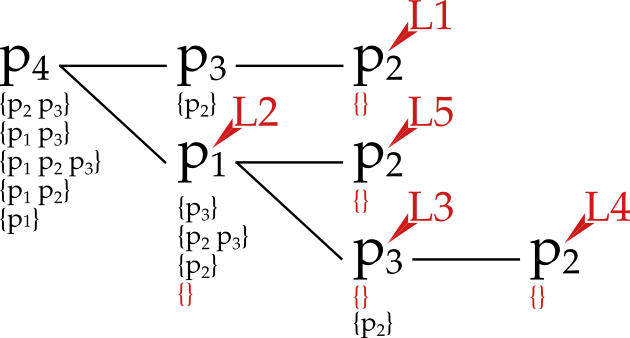
\includegraphics[scale=0.45]{figures/chapter7/advanced.png}
\caption{\label{fig:chap7_advanced} The trie with reduced width, representing all the labels of a compound entity in terms of involved properties. Each node is a property to explore. Attached to each node is the family of subsets that has to be decomposed. An empty set in a family related to a node (in red) signified that one of the initial subsets is fully represented in the trie, meaning that all the properties of a pattern will be explored by reaching this node. The width of the trie is three against five for the naive version.}
\end{figure}

In the following, such search-tree will be referred to as a \acrfull{ct}. Taking a part of it (i.e. taking one of its nodes as a local root) gives a sub-\acrshort{ct}.

\section{REG with compound relations}

Thanks to the \acrshort{ce} labels analysis, we have created a search-tree to lead the exploration of \acrshort{cr} in the \acrshort{reg} algorithm. In this section, we present the modification we made to use \acrshort{cr} in the \acrshort{reg} algorithm. The core of the algorithm based on the Uniform Cost Search algorithm is unchanged and is recalled in Algorithm~\ref{alg:chap7_ucs}.

\begin{algorithm}[!ht]
\caption{Uniform-Cost Search algorithm for Referring Expression Generation}
\label{alg:chap7_ucs}
\begin{algorithmic}
\Function{UCS\_REG}{$problem$} 
    \State $node\leftarrow$ a node with RE = \textsc{create-initial-re}(\textit{problem}.context), \textit{cost} = 0
    \State $frontier\leftarrow$ a priority queue of nodes ordered by their \textit{cost}
    \State $frontier\leftarrow$ \textsc{INSERT}($node$, $frontier$)
    \State $explored\leftarrow$ an empty set
    \Loop
        \If{\textsc{empty}($frontier$)} 
        	\State \Return failure
        \EndIf
        \State $node\leftarrow$ \textsc{pop}($frontier$)
        \If{\goaltest($problem$, \toquery($node$))} 
        	\State \Return \textsc{SOLUTION}($node$)
        \EndIf
        \State add $node.RE$ to $explored$
        \ForAll{$addition$ in \additions($node$)}
            \State $child \leftarrow \createchild(node, addition)$
            \If{$child.RE$ is not in $explored$ or $frontier$}
            	\State $frontier\leftarrow$ \textsc{INSERT}($child$, $frontier$)
            \EndIf
        \EndFor
    \EndLoop
\EndFunction
\end{algorithmic}
\end{algorithm}

\subsection{Exploring the compound relations}

At the difference of the taks descriptions of the previous chapter, the current algorithm can not have any prior knowledge about the relations leading to the use of \acrshort{cr}. A \acrshort{cr} can only be discovered if a relation introduces a \acrshort{ce}. However, an entity can be said to be a \acrshort{ce} only thanks to the labels of one of its upper class. With regard to this information, we cannot have any function dedicated to the addition of \acrshort{cr} and each newly introduced entity in a candidate \acrshort{re} has to be tested to assess if it is a \acrshort{ce} or not.


The analysis of the labels of entities and their usable classes (i.e. their upper classes having labels) is a process already existing in the \acrshort{reg} algorithm. It is performed by the function $\typingadditions$ of Algorithm~\ref{alg:typing_action}. It initially aims at satisfying the naming need constraint (theorem~\ref{the:parlance_need}). With some modifications, the $\typingadditions$ will be used to detect any newly introduced \acrshort{ce} by testing if the labels of the usable classes are in the form of a pattern. If they are, it returns the detected \acrshort{ce}. To do so, the \textit{additions} are now composed of a relation to be added and a \acrshort{ce} if one has been found.

\begin{algorithm}[b!]
\caption{\label{alg:chap7_child} Child node function modified to use compound relations.}
\begin{algorithmic}
\Function{\createchild}{$addition$, $parent$} 
    \State \Return a node with
    \State RE = $parent$.RE $\cup$ $addition$.relation
    \State cost = $parent$.cost + $\costfunc(addition$.relation$)$
    \If{$addition$.CE}
    	\State CTs $\leftarrow$ INSERT($\createtree(addition$.CE$)$, $parent$.CTs)
    \Else
    	\State CTs $\leftarrow$ $\getsubtrees$($addition$.relation, $parent$.CTs)
    \EndIf
\EndFunction
\end{algorithmic}
\end{algorithm}

Once \acrshort{ce}s have been detected, we have to create a \acrfull{ct} for each one in order to lead the \acrshort{reg} search process. To each node of the \acrshort{reg} algorithm, in addition to the candidate \acrshort{re} and its associated cost, we introduce a map of \acrshort{ct}s. This map links a \acrshort{ce} involved in the candidate \acrshort{re} related to the node to its \acrshort{ct} or one of its sub-\acrshort{ct}. The management of these trees is done by the $\createchild$ that has been modified (see Algorithm~\ref{alg:chap7_child}). If the addition introduces a new \acrshort{ce}, we create its related \acrshort{ct}\footnote{For performance gain, all created \acrshort{ct} can be stored in a collection of \acrshort{ct} in order to compute them only once even if the same \acrshort{ce} is introduced in two distinct branches of the \acrshort{ucs}.}. Otherwise, with the function $\getsubtrees$ we test if the new relation corresponds to one of the branches of one of the \acrshort{ct}s of the parent node. If it is, we take the sub-\acrshort{ct} corresponding to the relation. Taking the entity $\indiv_c$ as introduced \acrshort{ce} through the relation $(\indiv_4, \overline{\property_4}, \indiv_c)$, the \acrshort{ct} of Figure~\ref{fig:chap7_advanced} is first created. If in a second step the relation $(\indiv_c, \property_1, \indiv_1)$ is inserted, $\createchild$ would take the sub-\acrshort{ct} having $\property_1$ as root.

At this stage, we detect the introduction of \acrshort{cr} and manage the \acrshort{ct}s. The $\additions$ can now use the \acrshort{ct}s to propose new additions. As describe with Algorithm~\ref{alg:chap7_additions}, we keep the two functions $\typingadditions$ and $\differenceadditions$. We introduce a new function $\compoundadditions$ aiming to complete the \acrshort{cr} having been started. For each \acrshort{ct} of the node, it proposes the relation of the form $(\indiv_c, \property_i, \indiv_i) \in \relationset$ such that the properties $\property_i$ are the branches of the root of the \acrshort{ct} related to $\indiv_c$. With the  \acrshort{ct} of Figure~\ref{fig:chap7_advanced}, the $\compoundadditions$ function would generate two additions $(\indiv_c, \property_3, \indiv_3)$ and $(\indiv_c, \property_1, \indiv_1)$.

\begin{algorithm}[ht!]
\caption{\label{alg:chap7_additions} The modified $\additions$ function modified to use compound relations. }

\begin{algorithmic}

    \Function{\additions}{$node$} 
        \State $success, additions\leftarrow$ \typingadditions($node$)
        \If{$success = True\ and\ additions \neq \emptyset$}
            \Return $additions$
        \EndIf
        
        \State $additions\leftarrow$ \compoundadditions($node$) \Comment{new introduced function}
        \State $additions\leftarrow additions\ \cup$ \differenceadditions($node$) 
        
        \Return $additions$
    \EndFunction
    
\end{algorithmic}
\end{algorithm}

\subsection{Determining a referring expression validity}

Going back to the original definition of the \acrshort{reg} problem, a \acrshort{re} is valid if the naming need is satisfied (theorem~\ref{the:parlance_need}), all the introduced variables can be intantiated (theorem~\ref{the:correct_intance}), and the variable representing the target entity can only be bound to the target entity (theorem~\ref{the:re_mini_validity}) for a minimal validity.

For the compound relations, their validity criterion is that we can use one of their labels to speak about them. In other words, taking all the relations involving a given \acrshort{ce}, we must be able to rebuild one of its family's sets. Each of its \acrshort{cr} thus has to be complete (see theorem~\ref{the:cd_completion}).

\begin{theorem} [The CR completion]
\label{the:cd_completion}
A \acrshort{cr} of family $S$ is said to be complete iff given its \acrshort{ce} $\indiv_c$ we can create, from the set of relations $\mathcal{T}$ representing a candidate \acrshort{re}, a set $v = \{\property_i\ |\ (\indiv_c, \property_i, \indiv_i) \in \mathcal{T} \lor (\indiv_i, \overline{\property_i}, \indiv_c) \in \mathcal{T} \}$ such that $v \subset S$.
\end{theorem}

From a technical point of view, such a constraint can be hard to compute for each node to be tested. However, during the creation of a \acrshort{ct}, this information can already be known. During the \acrshort{ct} creation, each time a child node is created with an empty set as family of sets, this means that a label of the \acrshort{cr} is represented in its entirety at this node. In Figure~\ref{fig:chap7_advanced}, the completed labels are represented by the red arrows. We can thus store this information in the \acrshort{ct} nodes. Because during the \acrshort{reg} search process we cut down these trees taking each time a sub-\acrshort{ct}, we just have to test if each current root of the \acrshort{ct}s of the node to test can represent a label or not. If all of them can, the candidate \acrshort{re} of the current node is valid regarding the \acrshort{cr} completion.

\subsection{From tree to radix tree}

A limitation identified from the previous chapter was the addition of a single relation at each step while we can know that the candidate \acrshort{re} will not be valid because of the completion constraint. With the present method using multiple labels not involving all the relations, the limitation has been partially solved. In addition, thanks to the \acrshort{ct}, the branching factor is limited and even if an addition does not lead to a valid \acrshort{re}, it will be used for several labels. However, in some cases, this limitation still appears. Considering the \acrlong{ct} of Figure~\ref{fig:chap7_advanced}, starting from the root node $\property_4$, we can go to the nodes $\property_3$ and $\property_1$. While the node $\property_1$ creates a complete \acrshort{cr} and makes a step toward another complete \acrshort{cr}, the node $\property_3$ does not. It makes a step toward the single label $L1$ but does not complete it.

To solve this issue, we can use the radix tree structure, also called compact prefix tree. It consists of merging each node that is the only child with its parent if the parent node does not represent a valid label. In the example of Figure~\ref{fig:chap7_advanced}, the node with the property $\property_2$ could thus be merged with its parent $\property_3$.

The major consequence of such modification is that the additions have no more to represent a single relation but a set of relations. Even if it makes the additions comparison harder to compute it reduces the overall branching factor. Keeping our example, if we add at once the relation involving $\property_2$ and $\property_3$ and that both introduce an anonymous entity, this means that at the next step the $\typingadditions$ function could type both in one step. Where previously these additions would require four steps, and thus branching at each, with this solution it only requires two.

\section{Results}

In this section, we present some results of the \acrshort{reg} with compound relations. We start with the introduction example of Sean Connery's performance. Then we give performance measures using the setup of the previous chapter in order to assess the impact of the proposed modifications. 

\subsection{The actor playing James Bond}

For this simple test, we describe actor performance using the pattern of Figure~\ref{fig:chap7_perf}. Both the actor and the film can be used as a subject of the \acrshort{cr} thanks to the presence of inverse properties. The set of labels attached to the \textit{Performance} class is listed in Listing~\ref{lst:chap7_perf_labels}. Three are available to describe the actor and two (equivalent) for the film.

\newpage

\begin{figure}[ht!]
\centering
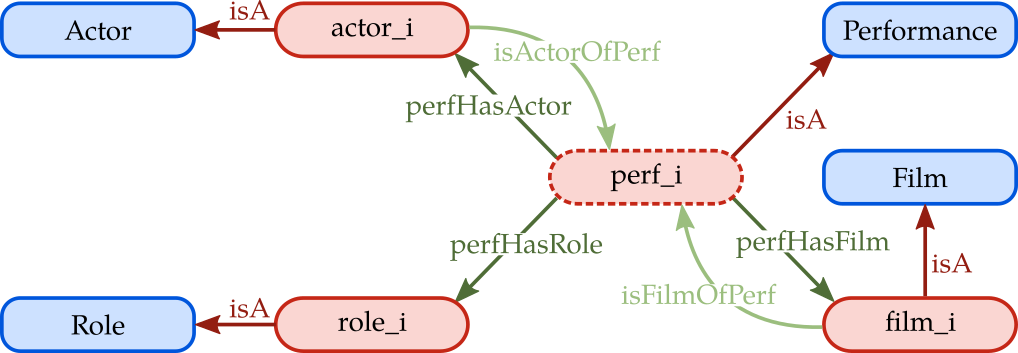
\includegraphics[scale=0.4]{figures/chapter7/perf.png}
\caption{\label{fig:chap7_perf} The compound relation pattern used to describe a performance of an actor with a role and a film.}
\end{figure}

\begin{lstlisting}[frame=single, caption={ The set of labels usable to describe the performance compound relation.}, label={lst:chap7_perf_labels}, captionpos=b, style=Labels, mathescape=true]
L1 - {?perfHasActor} who played {perfHasRole} in {perfHasFilm}
L2 - {?perfHasActor} who played {perfHasRole}
L3 - {?perfHasActor} who played in {perfHasFilm}
L4 - {?perfHasFilm} in which {perfHasActor} play {perfHasRole}
L5 - {?perfHasFilm} in which {perfHasRole} is played by {perfHasActor}
\end{lstlisting}

We first create an ontology describing two performances. The performance \textit{perf\_sean} link the actor \textit{sean\_connery} with the role of \textit{james\_bond} and the film \textit{gold\_finger}. The second is \textit{perf\_craig} with \textit{daniel\_craig} in the role of \textit{james\_bond} and in the film \textit{casino\_royale}. The individuals representing the films and the roles have labels while the others do not. Running our algorithm on this ontology we get the result:

\begin{gather*}
(?0,\ isA,\ Actor),\\
(?0,\ isActorOfPerf,\ ?1),\\
(?1,\ isA,\ Performance),\\
(?1,\ perfHasFilm,\ gold\_finger)
\end{gather*}

Matching it in the ontology, the variable \textit{?0} matchs \textit{sean\_connery} and the variable \textit{?1} matchs the performance \textit{perf\_sean}. Adding the performance \textit{perf\_gert} linking the actor \textit{gert\_frobe} with the role of \textit{auric\_finger} and the film \textit{gold\_finger} the previous solution is no more valid. Running the algorithm on the new ontology, we get the result:

\begin{gather*}
(?0,\ isA,\ Actor),\\
(?0,\ isActorOfPerf,\ ?1),\\
(?1,\ isA,\ Performance),\\
(?1,\ perfHasFilm,\ gold\_finger),\\
(?1,\ perfHasRole,\ james\_bond)
\end{gather*}

With this simple example we see that with a single compound relation, the algorithm is able to find a solution by selecting the necessary information in it depending on the situation, while keeping the link between each of them.

\subsection{The description of past activities as compound relations}

From now, we see that \acrlong{cr} can be used to represent complex knowledge with various entities linked together. Considering now the representation of an agent's past activities, presented in the previous chapter, such a complex knowledge could thus be represented using \acrshort{cr}s. Figure~\ref{fig:chap6_abox} represented a part of an ABox of an instance of a decomposition of the abstract task \textit{PrepareVegetable}. Focusing on the primitive task \textit{Cut} and its instance \textit{cut\_7}, we can observe that the underlying pattern already was a \acrshort{cr}. The graphical representation of this description is reported in Figure~\ref{fig:chap7_cut7}.

\begin{figure}[ht!]
\centering
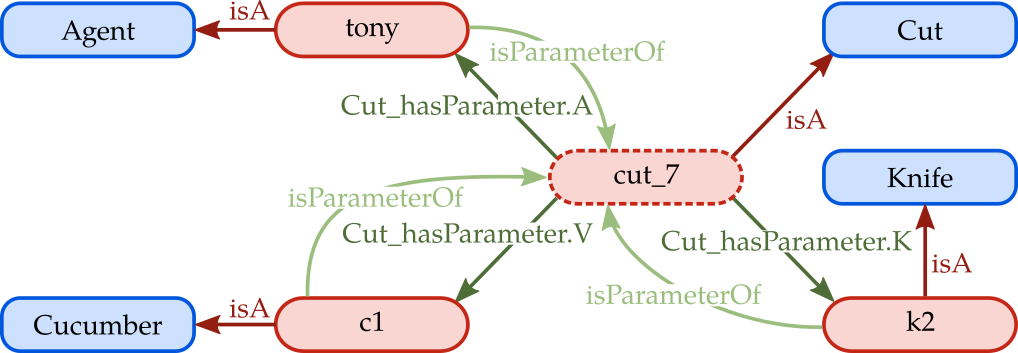
\includegraphics[scale=0.4]{figures/chapter7/cut7.png}
\caption{\label{fig:chap7_cut7} The underlined \acrlong{cr} pattern used to describe a past activity. The entity \textit{cut\_7} can thus be considered as a \acrlong{ce}. }
\end{figure}

At the light of the presentation of the \acrshort{cr}, we see that the entity \textit{cut\_7} is the \acrlong{ce} of the \acrlong{cr} and that the class \textit{Cut} is a relation class. Moreover, due to the presence of the inverse property \textit{isParameterOf}, common to all the used properties, the three involved entities could be used as a subject entity. The only element to add to the previous representation is the labels, in the form of patterns. For the cut task, the proposed labels are listed in Listing~\ref{lst:chap7_cut_labels}. Among these labels, we see that for all the possible subject entities, two labels are available, involving one or two additional entities.

\begin{lstlisting}[frame=single, caption={ The set of labels usable to describe the compound relation representing an instance of a cut primitive task.}, label={lst:chap7_cut_labels}, captionpos=b, style=Labels, mathescape=true]
L1 - {?Cut_hasParameter.A} who cut {Cut_hasParameter.V}
L2 - {?Cut_hasParameter.A} who cut {Cut_hasParameter.V} 
     with {Cut_hasParameter.K}
L3 - {?Cut_hasParameter.V} cut by {Cut_hasParameter.A}
L4 - {?Cut_hasParameter.V} cut by {Cut_hasParameter.A} 
     with {Cut_hasParameter.K}
L5 - {?Cut_hasParameter.K} with which {Cut_hasParameter.A} cut
L6 - {?Cut_hasParameter.K} with which {Cut_hasParameter.A} cut 
     {Cut_hasParameter.V}
\end{lstlisting}

To assess the utility to consider the past activities representation as \acrlong{cr}, we take again the execution trace of Figure~\ref{fig:chap6_meal_plan} and propose three new cases. The trace and the new cases are illustrated in Figure~\ref{fig:chap7_meal_plan}. As a reminder, the plan was executed by two agents, Tony, a human, and Pr2, a robot. A third agent, Bob, saw part of the execution. Each case corresponds to a set of tasks, seen and thus known by Bob. The goal here is still to refer to the knife \textit{k2}. The usable labels are thus L5 and L6, both referring to the knife used in the task.

\begin{figure}[ht!]
\centering
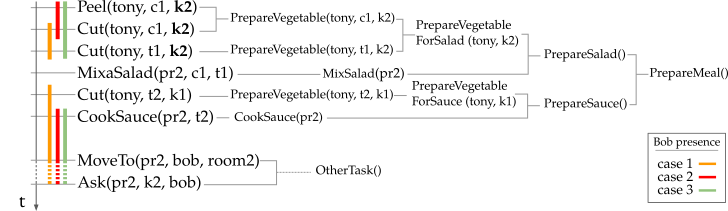
\includegraphics[width=\textwidth]{figures/chapter7/prepare_meal_plan.png}
\caption{\label{fig:chap7_meal_plan} The hierarchical execution trace to prepare the meal and a trace for another subsequent high-level task, organized according to a timeline. In the current instant, PR2 is asking Bob, a second human, for knife \textit{k2}. The three cases are represented by three colors at the left of the tasks and correspond to tasks seen by Bob, the human spectator.}
\end{figure}

\paragraph{Case 1:} Bob only saw two tasks involving the knife \textit{k2}. Both are cut tasks but on different vegetables. The algorithm can try to use the label L5, being shorter than L6. However, both tasks have been achieved by Tony. Consequently, the algorithm selects a \acrshort{re} using L6. The solution \acrshort{re} is: \textit{(?0 isA Knife), (?0 isParameterOf ?1), (?1 isA Cut), (?1 Cut\_hasParameter.A tony), (?1 Cut\_hasParameter.V ?2), (?2 isA tomato)}. The algorithm not based on \acrshort{cr}, would have given the same solution. The only difference is in its form. Here, the triplets representing the parameter use the properties really used to describe the \acrshort{cr}, where the previous algorithm would have used the more abstract property \textit{hasParameter}.

\paragraph{Case 2:} In the second case, Bob only saw two tasks involving the knife \textit{k2}. This time, it is two different tasks as one is a cutting task while the other is a peeling task. In this situation, the algorithm can use the label L5 and provide the solution: \textit{(?0 isA Knife), (?0 isParameterOf ?1), (?1 isA Cut), (?1 Cut\_hasParameter.A tony)}. We note that the cut vegetable is not present in the solution since it does not provide discriminative information. Bob saw Tony cut only a cucumber so specifying the vegetable would be useless. The algorithm not based on \acrshort{cr} would have provided all the parameters, even if some are useless. The \acrshort{cr}-based algorithm is thus able to find shorter \acrshort{re} when the current situation allows it.

\paragraph{Case 3:} In the third case, Bob saw three tasks. Two of them are cutting tasks while the other is a peeling task. Even if one of these tasks is different from the others, for the previous algorithm all of them involved three parameters. Consequently, they would have had all the same cost. The selection would have been based on the time, selecting the most recent one. For the \acrshort{cr}-based algorithm, the two cutting tasks need all of their parameters to be referred to but the peeling task can be used without reference to the peeled vegetable. Using the latter task allows to generate a shorter \acrshort{re}. Considering the peel task as having the same kind of labels than the cut task, the final solution \acrshort{re} is: \textit{(?0 isA Knife), (?0 isParameterOf ?1), (?1 isA Peel), (?1 Peel\_hasParameter.A tony)}.

Over these three cases, we saw the \acrshort{cr}-based algorithm is suitable to be used with descriptions of past activities. The advantage of this algorithm regarding the previously made is the form of the generated \acrshort{re} with the use of precise properties, and the ability to generate shorter \acrshort{re} in some situations. The most important point is that the algorithm is less dependant on the knowledge representation. It does not need a priori information about the properties of the representation. By simply adding labels to the existing representation, the current algorithm can be used with other task representations.

Finally, even if we will not illustrate it, the use of \acrshort{cr} to represent past activities could allow us to be restricted by the information provided by a task planned. Taking the example of the cut task, it is performed on a support, a work plan. Even if this piece of information is not necessarily provided by a task planner, when the task is performed, the work plan on which the task is performed can be perceived by the robot. This additional information could be used to generate \acrshort{re}. To support this new information, we could add a label L7:

\begin{quote} 
\centering 
\{?Cut\_hasParameter.K\} with which \{Cut\_hasParameter.A\} cut on \{TaskHasPlace\}
\end{quote}

With this new label, when a relation involving the property \textit{TaskHasPlace} exists, it would be explored and when it does not exist it would simply be discarded. This means that we can add additional and optional information to any \acrshort{cr}, and thus task representation.

\subsection{Assessing compound relations impact on performance}

Since the presented algorithm is able to manage the past tasks description, we present a comparison in terms of execution time with both the original algorithm and the one using past tasks. To do so, we take the \acrlong{kb} of the previous chapter (see Chapter~\ref{chap:6}) containing two tasks descriptions per entity inheriting from the \textit{Object} class. To be used with compound relations, we add a label to each class representing a task. The label involves the three parameters of the task. In this way, we reproduce the constraint to use all the parameters and at the same time take advantage of the radix-tree optimisations. The knowledge base is still managed using the Ontologenius system and not passing by the ROS services to not be impacted by the communication time in our measures.

\begin{figure}[ht!]
\centering
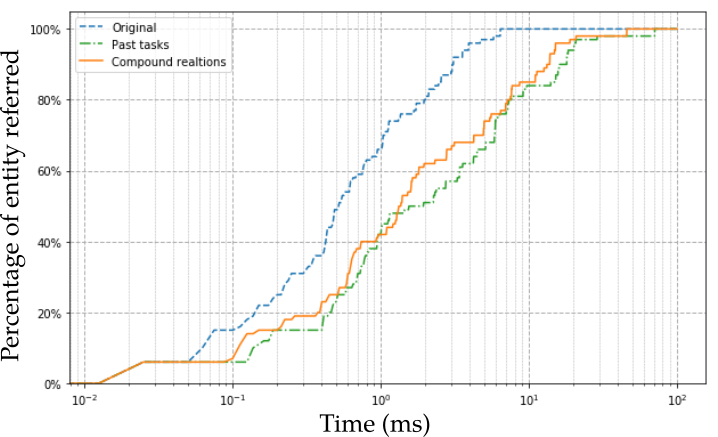
\includegraphics[scale=0.5]{figures/chapter7/comparison.png}
\caption{\label{fig:chap7_compare} Comparison of the three algorithms regarding the percentage of successfully referred entities over time using a logarithmic timescale. }
\end{figure}

The original algorithm has been run without the possibility to use relations toward task since it is not designed for this use. Its performance is our point of comparison as we expect all algorithms to find the same solutions. For the recall, the described tasks are designed in such a way to not help in the \acrshort{re} generation and but ourselves in the worst case. The measures of the percentage of entities referred over time for all three algorithms are represented in Figure~\ref{fig:chap7_compare} and reported on appendix~\ref{app:reg_comp_solutions}.

With this setup, the current version performs slightly better than the previous one with an average resolution time of 4.17ms versus 5.53ms. It is however more than the original version having an average resolution time of 1.08ms. This difference must be tempered by the exploration of \acrshort{cr}s that the original one does not do. While the majority of the entities are referred in a comparable time with the previous version, we can still note that the more complex entity requiring six relations is now solved in 45.71ms versus 70.57ms previously. \\

Here we have shown that the exploration of \acrshort{cr} has an impact, even if being acceptable with regards to \acrshort{hri} applications. However, the major advantage of this solution is that in case no \acrshort{cr}s are described in the \acrshort{kb}, no extra exploration is needed. This is a difference with the previous solution (see Chapter~\ref{chap:6}) where even if no tasks were described, the algorithm was trying to find some at each step. This means that, unlike the previous solution, if no \acrshort{cr}s are described in the \acrshort{kb}, the current solution has the same performance as the original version.

% chap 4
%count    77.000000
%mean      1.080750
%std       1.355236
%min       0.013237
%25%       0.193782
%50%       0.516371
%75%       1.322064
%max       6.405807

% chap 6
%count    77.000000
%mean      5.531283
%std       9.780631
%min       0.012952
%25%       0.509738
%50%       1.538461
%75%       5.968753
%max      70.577606

% chap 7
%count    77.000000
%mean      4.178141
%std       6.855033
%min       0.016902
%25%       0.438766
%50%       1.323878
%75%       5.447168
%max      45.716713
